


\tikzset{every picture/.style={line width=0.75pt}} %set default line width to 0.75pt

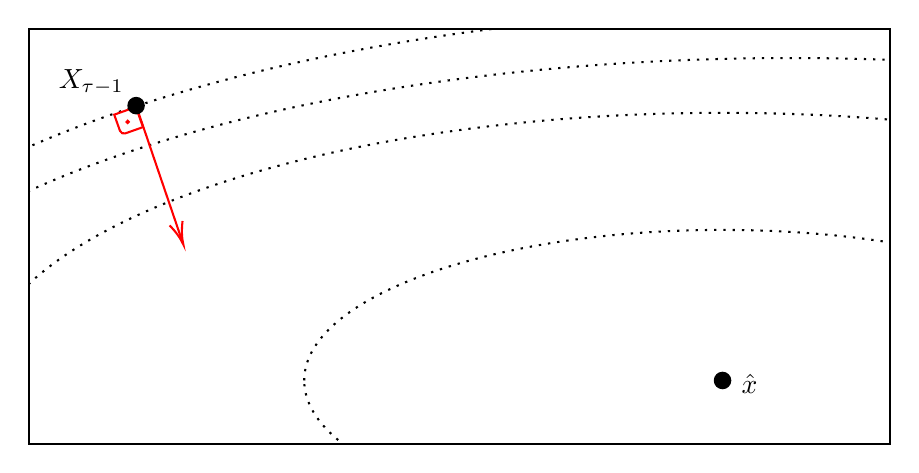
\begin{tikzpicture}[x=0.75pt,y=0.75pt,yscale=-1,xscale=1]
%uncomment if require: \path (0,221); %set diagram left start at 0, and has height of 221

\draw (150,10) rectangle (565,210);
\clip (150,10) rectangle (565,210);

%Shape: Ellipse [id:dp1243945339573651]
\draw  [dash pattern={on 0.84pt off 2.51pt}] (282.73,179.48) .. controls (282.73,139.42) and (372.97,106.94) .. (484.28,106.94) .. controls (595.59,106.94) and (685.83,139.42) .. (685.83,179.48) .. controls (685.83,219.55) and (595.59,252.02) .. (484.28,252.02) .. controls (372.97,252.02) and (282.73,219.55) .. (282.73,179.48) -- cycle ;
%Shape: Ellipse [id:dp7279543966183535]
\draw  [dash pattern={on 0.84pt off 2.51pt}] (126.02,179.48) .. controls (126.02,108.27) and (286.42,50.53) .. (484.28,50.53) .. controls (682.14,50.53) and (842.54,108.27) .. (842.54,179.48) .. controls (842.54,250.7) and (682.14,308.43) .. (484.28,308.43) .. controls (286.42,308.43) and (126.02,250.7) .. (126.02,179.48) -- cycle ;
%Shape: Ellipse [id:dp834765959265189]
\draw  [dash pattern={on 0.84pt off 2.51pt}] (49.52,192.48) .. controls (49.52,99.5) and (258.95,24.13) .. (517.28,24.13) .. controls (775.61,24.13) and (985.04,99.5) .. (985.04,192.48) .. controls (985.04,285.46) and (775.61,360.84) .. (517.28,360.84) .. controls (258.95,360.84) and (49.52,285.46) .. (49.52,192.48) -- cycle ;
%Shape: Ellipse [id:dp7198209862993796]
\draw  [dash pattern={on 0.84pt off 2.51pt}] (26.37,192.48) .. controls (26.37,86.13) and (255.37,-0.08) .. (537.86,-0.08) .. controls (820.34,-0.08) and (1049.34,86.13) .. (1049.34,192.48) .. controls (1049.34,298.83) and (820.34,385.05) .. (537.86,385.05) .. controls (255.37,385.05) and (26.37,298.83) .. (26.37,192.48) -- cycle ;
%Straight Lines [id:da9739335753395648]
\draw [color={rgb, 255:red, 255; green, 0; blue, 0 }  ,draw opacity=1 ]   (201.73,47.05) -- (223.88,112.15) ;
\draw [shift={(224.52,114.05)}, rotate = 251.20999999999998] [color={rgb, 255:red, 255; green, 0; blue, 0 }  ,draw opacity=1 ][line width=0.75]    (10.93,-3.29) .. controls (6.95,-1.4) and (3.31,-0.3) .. (0,0) .. controls (3.31,0.3) and (6.95,1.4) .. (10.93,3.29)   ;
%Shape: Ellipse [id:dp7361874596461209]
\draw  [fill={rgb, 255:red, 0; green, 0; blue, 0 }  ,fill opacity=1 ] (480.56,179.48) .. controls (480.56,177.43) and (482.23,175.76) .. (484.28,175.76) .. controls (486.33,175.76) and (488,177.43) .. (488,179.48) .. controls (488,181.53) and (486.33,183.2) .. (484.28,183.2) .. controls (482.23,183.2) and (480.56,181.53) .. (480.56,179.48) -- cycle ;
%Rounded Single Corner Rect [id:dp48113638837315853]
\draw  [color={rgb, 255:red, 255; green, 0; blue, 0 }  ,draw opacity=1 ] (196.58,60.42) .. controls (195.51,60.8) and (194.33,60.24) .. (193.95,59.17) -- (191.2,51.41) -- (201.62,47.71) -- (205.06,57.41) -- cycle ;
%Shape: Circle [id:dp7665286358613801]
\draw  [color={rgb, 255:red, 255; green, 0; blue, 0 }  ,draw opacity=1 ][fill={rgb, 255:red, 0; green, 0; blue, 0 }  ,fill opacity=1 ] (197.15,54.9) .. controls (197.15,54.61) and (197.38,54.38) .. (197.66,54.38) .. controls (197.95,54.38) and (198.18,54.61) .. (198.18,54.9) .. controls (198.18,55.18) and (197.95,55.41) .. (197.66,55.41) .. controls (197.38,55.41) and (197.15,55.18) .. (197.15,54.9) -- cycle ;

%Shape: Ellipse [id:dp6733708115016783]
\draw  [fill={rgb, 255:red, 0; green, 0; blue, 0 }  ,fill opacity=1 ] (198.02,47.05) .. controls (198.02,45) and (199.68,43.34) .. (201.73,43.34) .. controls (203.79,43.34) and (205.45,45) .. (205.45,47.05) .. controls (205.45,49.11) and (203.79,50.77) .. (201.73,50.77) .. controls (199.68,50.77) and (198.02,49.11) .. (198.02,47.05) -- cycle ;

% Text Node
\draw (492,175) node [anchor=north west][inner sep=0.75pt]    {$\hat{x}$};
% Text Node
\draw (163,28) node [anchor=north west][inner sep=0.75pt]    {$X_{\tau -1}$};

\end{tikzpicture}
